\documentclass[12pt,letterpaper]{beamer}
\usetheme{Copenhagen}
\usecolortheme{seahorse}
\setbeamertemplate{section in toc}{\inserttocsection}

\usepackage[utf8]{inputenc}
\usepackage{amsmath}
\usepackage{amsfonts}
\usepackage{amssymb}
\usepackage{graphicx}
\graphicspath{ {./images/} }
\usepackage{multirow}
\usepackage{hyperref}
\hypersetup{
    colorlinks=true,
    linkcolor=blue,
    filecolor=magenta,      
    urlcolor=cyan,
    pdftitle={Overleaf Example},
    pdfpagemode=FullScreen,
}
\usepackage{minted}

\title[Robotics I]
{ENGR 3421: ROBOTICS I}
\subtitle{Encoder}

\author[Zhang, Lin]
{Dr. Lin Zhang}
\institute[UCA] % (optional)
{
  Department of Physics and Astronomy\\
  University of Central Arkansas
}
\date[Robotics1 2021] % (optional)
{September 28, 2021}
\logo{
\includegraphics[height=1cm]{../images/uca_bear_logo.png}}


%End of title page configuration block
%------------------------------------------------------------

%------------------------------------------------------------
%The next block of commands puts the table of contents at the beginning of each section and highlights the current section:

% \AtBeginSection[]
% {
  % \begin{frame}
    % \frametitle{Outline}
    % \tableofcontents[currentsection]
  % \end{frame}
% }
% %------------------------------------------------------------
% 
\begin{document}

%The next statement creates the title page.
\frame{\titlepage}
% 
% %---------------------------------------------------------
% %This block of code is for the table of contents after the title page
% \begin{frame}
% \frametitle{Outline}
% \tableofcontents
% \end{frame}
%---------------------------------------------------------

\begin{frame}{Types of Encoder}

\centering
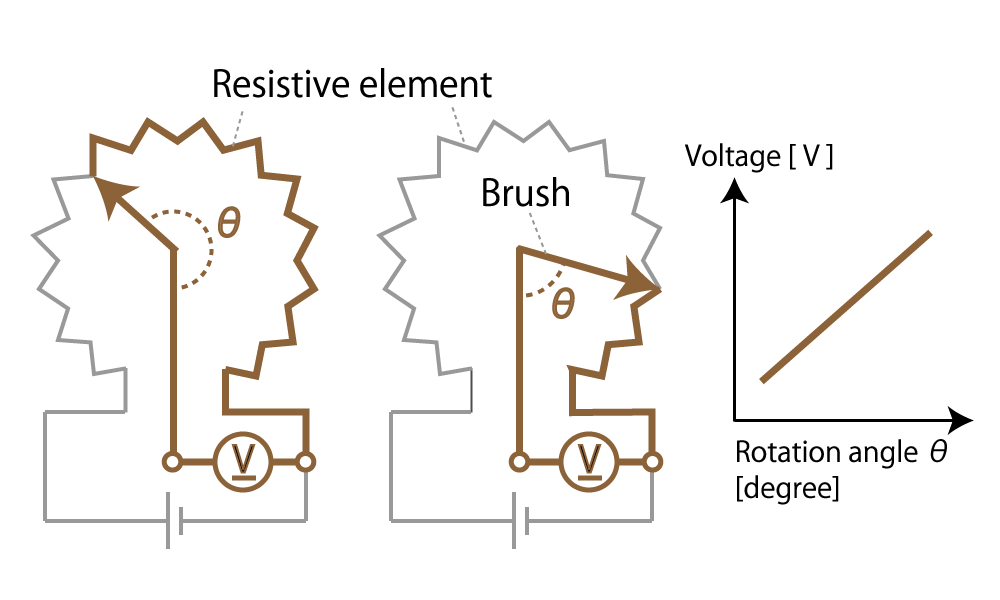
\includegraphics[width=0.4\textwidth]{mechanical_encoder}
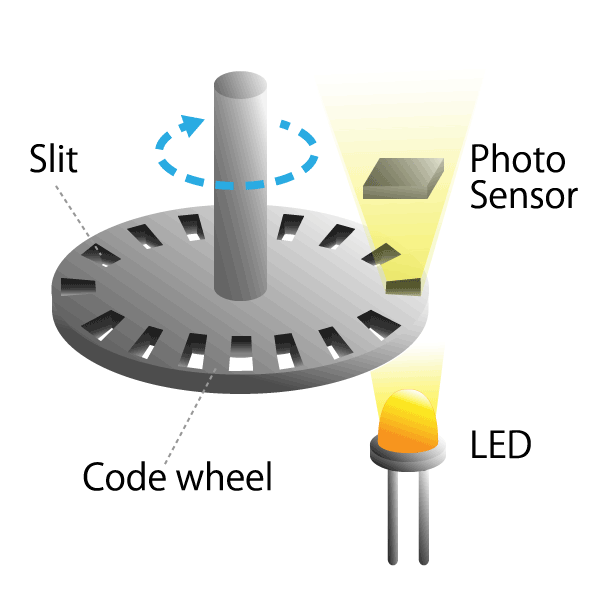
\includegraphics[width=0.4\textwidth]{optical_encoder}
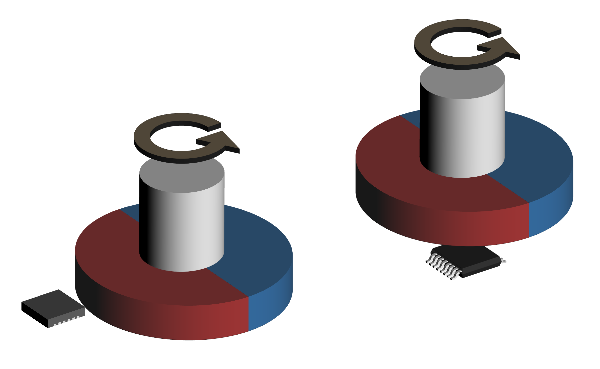
\includegraphics[width=0.4\textwidth]{magnetic_encoder}
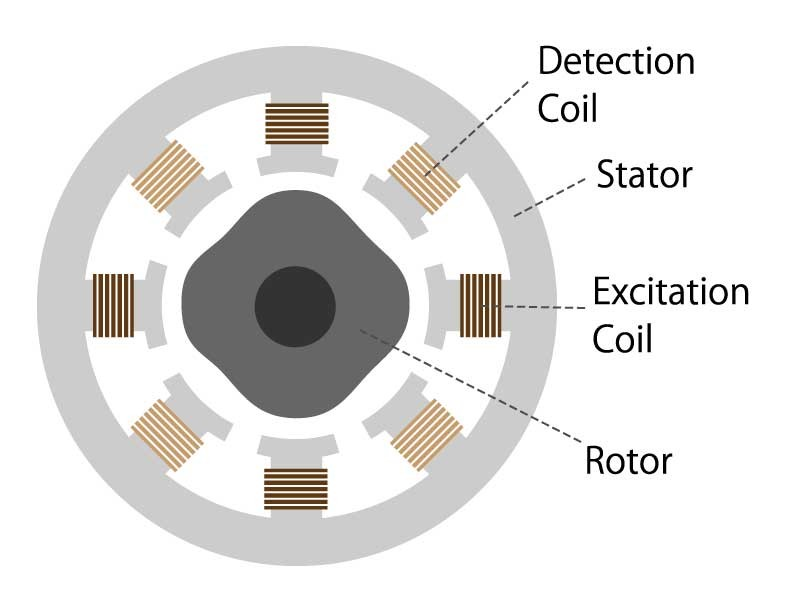
\includegraphics[width=0.4\textwidth]{electromagnetic_encoder}

\end{frame}

\begin{frame}{Hall Effect}

\centering
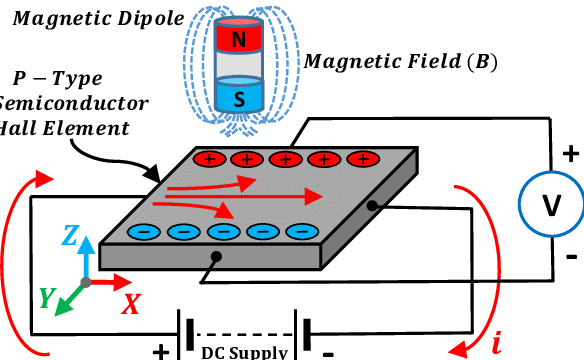
\includegraphics[width=0.8\textwidth]{hall_effect}

\end{frame}

\begin{frame}{Absolute Encoder vs. Incremental Encoder}

    \centering
    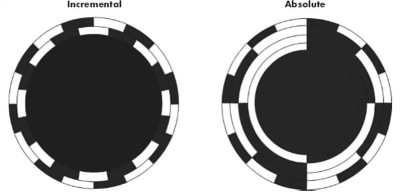
\includegraphics[width=0.6\linewidth]{absolute_incremental}

    {\scriptsize
    \begin{tabular}{ cc }
        \hline
        \textbf{Absolute} & \textbf{Incremental} \\
        \hline
        More complicated & Simpler \\
        Output position and velocity & Output velocity and displacement (optionally direction) \\
        Fixed origin & Floating origin \\
        Lower cost & More expensive \\
        \hline
    \end{tabular}
}
    
\end{frame}

\begin{frame}{Quadrature Encoder}
    
    \centering
    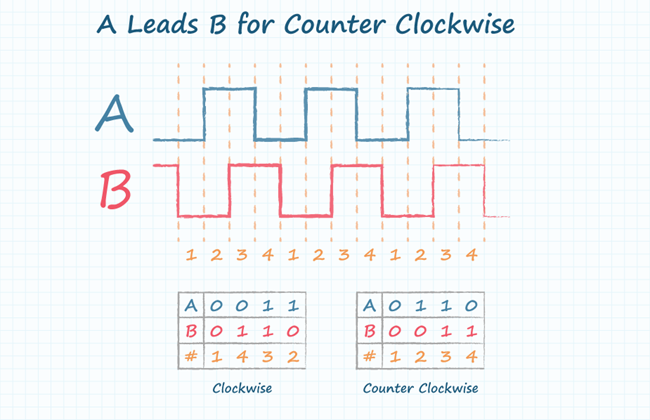
\includegraphics[width=0.8\linewidth]{quadrature}

\end{frame}


\end{document}



